%!TEX root = francis_thesis.tex
%%%%%%%%%%%%%%%%%%%%%%%%%%%%%%%%%%%%%%%%%%%%%%%%%%%%%%%%%%%%%%%%%%%%%%%
\chapter{Results and analysis}\label{ch:Results}


\section{Used Technologies}
Various technologies, frameworks and libraries were used in this project. Every implementation was carried out in Python, and frameworks like TensorFlow and Keras were used. Below are the list of the technologies used and a brief description.

\subsection{Python}

\begin{figure}[H]
    \centering
    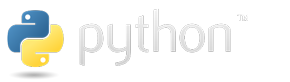
\includegraphics[width=0.8\linewidth]{images/python-logo.png}
     \caption{Python logo, source: https://www.python.org/community/logos/}
  \end{figure}

Python\footnote{https://www.python.org/community/logos/} is a high level programming language designed by Guido van Rossum in 1991. Its design philosophy emphasizes code readability and has a remarkable use of significant whitespace. The filename extensions include .py, .pyc, .pyw, .pyz. It support web development with frameworks like Django and Pyramid. It is applied in scientific studies and machine learning. Several libraries and frameworks have been developed by the Python community for this such as 
SciPy\footnote{www.scipy.org}, Scikit-learn\footnote{scikit-learn.org/stable/}, Pandas\footnote{pandas.pydata.org}, Numpy\footnote{www.numpy.org/}, Theano\footnote{deeplearning.net/software/theano/}, PyTorch \footnote{pytorch.org/}, etc. It is also one of the most popular languages in the field of Convolutional neural network. Neural Networks like ResNet, VGGNet, Faster R-CNN, AlexNet in Keras or Pytorch, etc. 

\subsection{ TensorFlow}
\begin{figure}[H]
    \centering
    
\includegraphics[width=0.7\linewidth]{images/TensorFlow.png}
     \caption{TensorFlow logo, source: www.tensorflow.org}
  \end{figure}
TensorFlow\footnote{www.tensorflow.org} is an Apache Licensed library. It is free and open-sourced and developed by Google Brain Team. It is written in Python, C++ and CUDA. It is a symbolic math library applied for machine learning application such as deep neural network, convolutional neural network. TensorFlow was used in the implementation of the deep learning network for this project. TensorFlow has a comprehensive, flexible ecosystem of tools, libraries that makes it user-friendly.
For a wider documentation, please see the official website\footnote{www.tensorflow.org}
\clearpage

\subsection{Keras}
\begin{figure}[H]
    \centering
    
\includegraphics[width=0.9\linewidth]{images/keras.png}
     \caption{Keras logo, source:www.scikit-image.org}
  \end{figure}

Keras \footnote{Keras.io} is an MIT licensed neural-network library written in Python. It was design by Francois Chollet and released first in March 2015. It is open-sourced. Keras is capable of running on top of Microsoft Cognitive Toolkit, TensorFlow, PlaidML or Theano for fast experimentation of deep neural networks. It enables implementation of deep learning and allows easy and 
fast prototyping, supports both convolutional networks and recurrent networks and the combination of both. For a wider documentation, please see the official website\footnote{www.keras.io}

\subsection{ Scikit-Image}
\begin{figure}[H]
    \centering
    
\includegraphics[width=0.7\linewidth]{images/Scikit-image.png}
     \caption{Scikit-Image logo, source: www.scikit-image.org}
  \end{figure}

Scikit-Image is a BSD licensed image processing library. It is a collection of algorithms for segmentation, 
geometric transformations, analysis, filtering, colour space manipulation, morphology, feature detection, and so on. It was first released in 2009, written by Stefan van der Walt.
\section{Implementation}
\subsection{Dataset}
Drones, or general UAVs, equipped with cameras have been fast applied to a wide range of applications, including agricultural, aerial photography, fast delivery, and surveillance. Consequently, automatic understanding of visual data collected from these platforms become highly demanding, which brings computer vision to drones more and more closely. 
Various computer vision task has been carried out by the Vision meets Drone (VisDrone) Challenges\footnote{www.aiskyeye.com}
organized  by the AISKEYE team at Lab of Machine Learning and Data Mining , Tianjin University, China in the year 2018.
Various computer vision task carried out in the challenge include object detection in images. The task aims to detect objects of predefined categories (e.g., cars and pedestrians) from individual images taken from drones. Also, object detection in videos challenge. The task is similar to the first, except that objects are required to be detected from videos. Then single-object tracking challenge. The task aims to estimate the state of a target, indicated in the first frame, in the subsequent video frames. And finally, multi-object tracking challenge. The task aims to recover the trajectories of objects in each video frame.
Originally, I wanted to use the dataset provided by VisDrone Challenge for the training and validation of my Mask R-CNN Network, but due to lack of the segmentation mask data for the training set, I couldn’t use it.
Rather I made use of the Semantic Drone Dataset from Institute of Computer Graphics and Vision, Graz University of Technology, Austria. \footnote{dronedataset.icg.tugraz.at}

\paragraph{}
The dataset contains images, bounding boxes as python pickle file, bounding boxes as xml, bounding boxes as mask images. The Semantic Drone Dataset focuses on semantic understanding of urban scenes for increasing the safety of autonomous drone flight and landing procedures. The imagery depicts  more than 20 houses from nadir (bird's eye) view acquired at an altitude of 5 to 30 meters above ground. A high resolution camera was used to acquire images at a size of 6000x4000px (24Mpx). The training set contains 400 publicly available images and the test set is made up of 200 private images. [W]
For the task of person detection the dataset contains bounding box annotations of the training and test set. And for semantic segmentation, pixel-accurate annotation for the same training and test set was prepared. The complexity of the dataset is limited to 20 classes as listed below.

\begin{itemize}
  \item tree
  \item tree
  \item grass
  \item other vegetation
  \item dirt
  \item gravel
  \item rocks
  \item water
  \item paved area
  \item pool
  \item person
  \item dog
  \item car
  \item bicycle
  \item roof
  \item wall
  \item fence
  \item fence-pole
  \item window
  \item door
  \item obstacle
  
\end{itemize}
The Drone Dataset is made freely available to academic and non-academic entities for non-commercial purposes such as academic research, teaching, scientific publications, or personal experimentation.
\paragraph{}
For the implementation of the instance segmentation, Python was used for obvious reasons. It enabled me to use deep learning framework like Tensorflow and Keras. The implementation of the model was carried out in the file drone.py and uses the Mask R-CNN library developed in python with TensorFlow and Keras by Matterport Inc. It was written by Waleed Abdulla from Matterport Inc. Matterport, Inc. published their implementation under the MIT License [X]. The MIT License is a license granting the permission to use the code, copy it, modify it, publish and even to sell it free of charge.
There's absolutely no restriction on commercial use in MIT license. The only requirement is that you must include the MIT copyright notice with any copies of the software. Scripts, files and noteboks in the library are also under the MIT License and moreover, Waleed Abdulla himself agreed with the usage and modifications of his code for purposes of the research work.The Matterport, Inc. Mask R-CNN implementation can be found in their GitHub repository.
Moreover, the Matterport implementation of Mask R-CNN was selected because of several reasons. Besides its license compatibility, it is quite robust and ready for modifications and adaptation for training in drone dataset leading to another implementation, so it saved thousands of lines of code. One of the major motivation behind its usage is that there is a plenty of people interested in this project, proposing their ideas and testing it. And these people are experienced in fields of computer vision and deep learning. Abdulla himself is responsive and active in answering people’s questions and issues. He is open-minded when discussing other people improvement proposals. I found it very useful.
The next section will discuss the Mask R-CNN library, the workflow and necessary module of the library. The structure, architecture and components of the Mask R-CNN have been discussed in Chapter 2, so explanation of the programs only will be given in the next section. The library will be also discussed altogether with notes on my modifications connected with this thesis to distinguish them from Abdulla’s code.

\subsection{Mask R-CNN library}
The library which is hosted in Github has been forked 5445 times. It contains five important modules. Each module play an important role in the training and testing of model. Let’s go through this modules on after the other below:
\textbf{Config.py}
This is the configuration module of the system. It includes hyper-parameters for tuning of the model and necessary setting. It will described in section 4.2.1
\textbf{Model.py}
This is fundamental core of the model. It develops and builds up the model. It will described in section 4.2.2	
\textbf{Parallel\_Model.py} 
This module subclasses the standard Keras Model and adds multi-GPU support. It works by creating a copy of the model on each GPU and creates a parallelized computation.
This file was not modify further and so will not explained in this thesis.
\textbf{Utils.py} 
This modules contains the utility classes and functions of the model. It will described in section 4.2.3
\textbf{Visualize.py}
This contains function for display and visualization. It will described in section 4.2.4

The python files for the modules have good inner documentation, of which some of them and other functionalities will be discussed next.

\subsubsection{Config.py}
Config.py is the configuration settings for the model in the implementation by Matterport Inc.. It contains the hyper-parameters of the model. It has a classed called ModelConfig that houses these parameters. These parameter include;
 \begin{itemize}
   \item GPU Count
   \item Images per GPU
   \item Steps per Epoch
   \item Validation steps
   \item The choice of the backbone
   \item Backbone strides (The strides of each layer of the Feature Pyramid Network (FPN) pyramid discussed in section 2.2)
   \item Learning Rate
   \item RPN Train Anchors Per\_ Image (How many anchors per image to use for RPN training)
   \item Mask Shape
   \item And so on.
   
 \end{itemize}
 I inherited ModelConfig  class and then adapted the attributes to suit my hardware and the drone-based dataset in the drone.py module.  The config.py also a contains a display function that displays the model’s attribute.

 \subsubsection{Model.py}
 This is the main Mask R-CNN implementation. It is made use of some modules for its implementation which include, os, random, datetime, re, logging, collections, multiprocessing ,numpy,tensorflow, keras, keras.backend ,keras.layers ,keras.engine , ,keras.models. distutils.version. For the module to work it needs TensorFlow 1.3+ and Keras 2.0.8+ .  Since this module builds the Mask R-CNN it has several classes and function performing various tasks. This classes and task the perform can be summed up thus;
 \begin{itemize}
   \item 	Initialization functions
   \item Building the ResNet backbone.
   \item Building the RPN.
   \item Building RoIAlign layers.
   \item Building head architectures.
   \item Building the complete Mask R-CNN model and putting everything together.
   \item Building detection layers.
   \item Defining loss functions.
   \item	Data formatting
   \item Miscellaneous functions and utilities connected to the model, like batch normalization data formatting and generating (building up targets, loading ground truth masks) or bounding boxes normalization.
   
 \end{itemize}
 Some important functions in the modules include train, load\_weight, build, etc. There was no modification made in this module for the training of model, apart from few modification to fix error that could be raised during the loading of masks. An explanation is given to the program written by Waleed Abdulla 